\documentclass[11pt, a4paper]{article}
% Shared preamble for the methodology and validation reports.
%
% siunitx is loaded conditionally. It is standard in TeX Live and MacTeX, but
% absent from minimal Debian installations, and these documents must compile in
% continuous integration as well as on a workstation. The fallbacks reproduce
% only the commands used here.
\usepackage[a4paper, margin=25mm]{geometry}
\usepackage{amsmath}
\usepackage{booktabs}
\usepackage{tikz}
\usepackage{pgfplots}
\usepackage{subcaption}
\usepackage{graphicx}
\usepackage[hidelinks]{hyperref}

\usetikzlibrary{arrows.meta, positioning}
\pgfplotsset{compat=1.18}

% A conditional is used rather than the false branch of \IfFileExists because
% a macro parameter (#1) written inside another macro's argument is consumed
% during expansion, producing "Illegal parameter number".
\newif\ifhassiunitx
\IfFileExists{siunitx.sty}{\hassiunitxtrue}{\hassiunitxfalse}

\ifhassiunitx
  \usepackage{siunitx}
  \sisetup{detect-all, per-mode=symbol}
\else
  \typeout{NOTE: siunitx unavailable; using minimal fallbacks.}
  \providecommand{\num}[1]{\ensuremath{#1}}
  \providecommand{\si}[1]{\ensuremath{\mathrm{#1}}}
  \providecommand{\qty}[2]{\ensuremath{#1\,\mathrm{#2}}}
  \providecommand{\degree}{^{\circ}}
\fi

\newcommand{\code}[1]{\texttt{#1}}
\setlength{\parskip}{0.4em}
\setlength{\parindent}{0pt}


\title{Relief Forge Tools: Validation}
\author{Synthetic test geometry and measured accuracy}
\date{}

\begin{document}
\maketitle

\begin{abstract}
This document records how the geometry operations in this repository are
verified. Every test case is constructed in closed form, so expected values
derive from geometry rather than from a previous run of the code under test.
All tables are generated from live execution by \code{docs/make\_tables.py} and
\code{scripts/benchmark.py}; none are transcribed by hand.
\end{abstract}

\section{Synthetic test geometry}

The test suite uses no binary assets. Every fixture is built analytically at
run time, which makes the suite deterministic, fast, and executable without
network access, model weights or a GPU. Fixtures fall into three groups.

\textbf{Valid solids.} A closed axis-aligned cube provides the reference case:
its volume, surface area, edge count and mean dihedral angle are all known
exactly. An annulus --- a washer with a through hole --- provides a valid solid
of genus one, confirming that no check incorrectly assumes a simply connected
surface. A subdivided octahedron approximates a sphere and provides a case
where the expected value is approached rather than met exactly.

\textbf{Defect fixtures.} Each is the reference cube with exactly one defect
introduced, so a detection failure localises immediately: one face removed
produces boundary edges; one triangle reversed produces inconsistent winding; a
two-triangle flap attached to an existing edge produces a non-manifold edge;
two separated cubes produce a second connected component; and reversing every
triangle produces negative signed volume while leaving the surface closed.

\textbf{Symmetry fixtures.} A box spanning $x \in [-10, 5]$ exercises an
off-centre cut with a known result. A sphere displaced along $x$ exercises a
cut whose expected volume follows from the spherical-cap formula. The annulus
exercises the case where vertices lie exactly on the cut plane.

\section{Analytical expected values}

Expected values are closed-form wherever the geometry permits. For the cube of
edge $a$: $V = a^3$, $A = 6a^2$. For the annulus of outer radius $R$, inner
radius $r$ and height $h$:
%
\begin{equation}
  V = \pi \left( R^2 - r^2 \right) h,
  \qquad
  A = 2\pi \left( R + r \right) h + 2\pi \left( R^2 - r^2 \right)
\end{equation}
%
For the symmetrized displaced sphere, the retained portion is a spherical cap
of height $h = R - d$ on a sphere of radius $R$ displaced by $d$; the mirrored
result is two such caps:
%
\begin{equation}
  V = 2 \cdot \frac{\pi h^2 \left( 3R - h \right)}{3}
\end{equation}

The cube's mean dihedral angle is obtained by counting rather than by
formula. A cube tessellated as two triangles per face has 18 unique edges: 12
geometric edges at \qty{90}{\degree} and 6 face diagonals at
\qty{0}{\degree}, giving a mean of exactly \qty{60}{\degree}. This is a strong
test, since an error in edge pairing changes the count and therefore the mean.

Table~\ref{tab:measurements} reports measured values against these
expectations.

\begin{table}[h]
  \centering
  \small
  % Generated by docs/make_tables.py. Do not edit by hand.
\begin{tabular}{lrrrrr}
\toprule
Quantity & Unit & Expected & Measured & Rel.\ error & Tolerance \\
\midrule
Cube volume & mm$^3$ & 1\,000.0000 & 1\,000.0000 & \num{0.00e+00} & \num{1e-09} \\
Cube surface area & mm$^2$ & 600.0000 & 600.0000 & \num{0.00e+00} & \num{1e-09} \\
Cube mean dihedral angle & deg & 60.0000 & 60.0000 & \num{0.00e+00} & \num{1e-09} \\
Cube cast mass, silver 925 & g & 10.3600 & 10.3600 & \num{0.00e+00} & \num{1e-09} \\
Annulus volume & mm$^3$ & 791.6813 & 790.4102 & \num{1.61e-03} & \num{3e-03} \\
Annulus surface area & mm$^2$ & 791.6813 & 790.7280 & \num{1.20e-03} & \num{3e-03} \\
Sphere volume & mm$^3$ & 2\,144.6606 & 2\,141.5041 & \num{1.47e-03} & \num{1e-02} \\
Symmetrized sphere volume (cap formula) & mm$^3$ & 1\,357.1680 & 1\,354.7132 & \num{1.81e-03} & \num{2e-02} \\
Symmetrized box volume & mm$^3$ & 960.0000 & 960.0000 & \num{0.00e+00} & \num{1e-09} \\
\bottomrule
\end{tabular}
  \caption{Measured values against analytical expectations. Relative error and
  the tolerance applied by the test suite are shown for each quantity.}
  \label{tab:measurements}
\end{table}

\section{Numerical tolerances}

Two tolerance regimes apply, and the distinction is deliberate.

\textbf{Exact cases} use a relative tolerance of $10^{-9}$. The cube's volume,
surface area and mean dihedral angle, and the symmetrized box's volume, are
representable in double precision without accumulation error; the summations
involved are short and well conditioned. A tolerance this tight would fail on
any error in the algorithm rather than in floating point.

\textbf{Discretisation cases} use tolerances matched to a known approximation
error. The annulus is a 64-segment polygonal approximation of a circle. Its
outline is inscribed, so it under-estimates the true area by a factor of
$\operatorname{sinc}(1/n) \approx 1 - \pi^2/(6n^2)$, about \num{8e-4} at
$n = 64$. The tolerance is set at \num{3e-3}, comfortably above that bound but
far below any plausible algorithmic error. The test additionally asserts that
the measured volume is \emph{less} than the exact value, which verifies the
sign of the discretisation error rather than only its magnitude.

The subdivided-octahedron sphere is likewise inscribed and converges more
slowly, so it carries a \num{1e-2} tolerance, and the symmetrized sphere
\num{2e-2}, reflecting the compounding of two approximations.

Stating tolerances by regime rather than using one loose global value means a
tightening of the discretisation cannot silently mask a regression in the
exact cases.

\section{Failure detection}

Table~\ref{tab:defects} records what the analysis reports for each fixture.
Each defect fixture must be detected as exactly its own defect, and the valid
solids must produce no false positives --- including the annulus, whose through
hole is valid geometry and must not be reported as a defect.

\begin{table}[h]
  \centering
  \small
  % Generated by docs/make_tables.py. Do not edit by hand.
\begin{tabular}{lll}
\toprule
Fixture & Injected defect & Detected \\
\midrule
Closed cube & none & none \\
Cube, one face removed & open surface & 4 boundary \\
Cube, one triangle reversed & winding & 3 winding \\
Cube with attached flap & non-manifold & 3 boundary, 1 non-manifold \\
Two separated cubes & disconnected & 2 components \\
Annulus (genus one) & none & none \\
Inverted cube & orientation & negative volume \\
\bottomrule
\end{tabular}
  \caption{Injected defects and the classification reported by the analysis.}
  \label{tab:defects}
\end{table}

\begin{figure}[h]
  \centering
  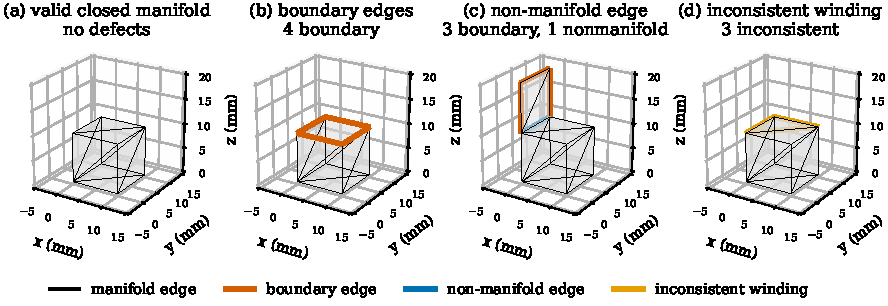
\includegraphics[width=\textwidth]{../figures/generated/fig_topology_diagnostics.pdf}
  \caption{Edge classification on synthetic meshes. Defective edges are drawn
  in the colour of their classification; all four panels share one camera and
  one set of axis limits.}
  \label{fig:topology}
\end{figure}

Two failure modes deserve specific mention because they are easy to miss.

An \textbf{inverted mesh} --- every triangle reversed --- is a closed manifold
and passes every edge-incidence test. Only the sign of the signed volume
distinguishes it from a valid solid. This is why orientation is checked
independently of topology rather than inferred from it.

\textbf{Disconnected solids} are each individually valid. Two separated cubes
have no boundary edges, no non-manifold edges and consistent winding
throughout. Only the component count reveals the condition, which is why the
expected component count is an explicit parameter rather than an assumption.

\subsection{A defect found by these tests}

The plane-intersection cases were added after the symmetry operation produced a
non-manifold result on the annulus. Vertices of that fixture lie exactly on the
cut plane, and three degenerate cases followed: triangles lying wholly in the
plane were duplicated by their own mirror image; triangles on the discarded
side touching the plane at one vertex clipped to zero-area slivers; and
intersections computed at vertices already on the plane repeated points in the
output polygon. The current implementation handles all three, and the annulus
case is retained specifically to prevent regression.

\section{Performance}

Table~\ref{tab:benchmark} reports measured timings across synthetic mesh sizes.
Values come from actual runs on the machine and software versions recorded in
the table's source file; they are not estimates and are not transferable to
other hardware.

\begin{table}[h]
  \centering
  \small
  % Generated by scripts/benchmark.py. Do not edit by hand.
\begin{tabular}{rrrrrrr}
\toprule
Triangles & File (MB) & Parse (ms) & Weld (ms) & Topology (ms) & Total (ms) & Peak mem.\ (MB) \\
\midrule
512 & 0.024 & 0.01 & 0.40 & 3.07 & 3.49 & 0.21 \\
2\,048 & 0.098 & 0.02 & 1.53 & 12.36 & 13.91 & 0.74 \\
8\,192 & 0.391 & 0.04 & 6.62 & 50.66 & 57.33 & 2.96 \\
32\,768 & 1.563 & 0.18 & 27.51 & 207.86 & 235.56 & 11.82 \\
\bottomrule
\end{tabular}

% environment: Linux-6.8.0-124-generic-aarch64-with-glibc2.35, python 3.10.12, numpy 2.2.6, measured 2026-07-26 22:26:23
  \caption{Measured cost of parsing, welding and topology analysis. Median of
  five runs per configuration.}
  \label{tab:benchmark}
\end{table}

Topology analysis dominates, and its cost is superlinear in triangle count
because connected-component labelling uses a Python-level union-find loop while
parsing and welding are vectorised. This is the obvious optimisation target
should larger meshes become routine; it has not been undertaken because meshes
at the scale this pipeline produces are analysed in well under a second.

\section{Known limitations}

\textbf{Scope of the checks.} A mesh passing validation has no boundary edges,
no non-manifold edges, no degenerate edges, consistent local winding, positive
signed volume, and the expected component count. This establishes that it is a
closed, coherently oriented solid. It does not assess minimum wall thickness,
unsupported overhangs, printer tolerances, casting shrinkage, trapped volumes,
or any process-specific constraint.

\textbf{Self-intersection is not detected.} A surface may be closed, manifold
and correctly wound while passing through itself. Detecting this requires
pairwise triangle intersection tests, which are not implemented.

\textbf{Welding tolerance is heuristic.} Vertices closer than the tolerance are
merged. On a mesh with genuine detail below that scale, welding could join
surfaces that should remain distinct. The default of $10^{-6}$ of the
bounding-box diagonal is far below the resolution of any casting process, but
it is a choice rather than a derived bound.

\textbf{Mean dihedral angle is a limited proxy.} It is interpretable only when
comparing closely related meshes of the same object at identical scale and
comparable triangle density. It is not a perceptual quality metric and carries
no meaning across unrelated meshes or across tessellation densities.

\textbf{Material mass assumes a dense solid.} Equation~$m = \rho|V|$ excludes
sprue, flashing and shrinkage, and alloy densities vary between suppliers. The
estimate supports comparison between candidate geometries; it does not certify
a finished part.

\textbf{Generation is not covered by these tests.} The test suite validates
geometry processing only. Backend inference requires model weights, a GPU and
network access, and is therefore excluded from automated testing.

\end{document}
